\chapter{Case study}
\label{chap:case_study}

\section{Overview}

The goal of this chapter is to present a case study of a hierarchical runtime verification technology based on the previous chapters. The motive of this study is the related report from 2014 \citep{tdk2014}, which goal was a distributed, model based security logic. Their case study called the \emph{Model Railway Project}, and our study integrates their work, and finds ways to integrate it with other sensor sources for a hierarchical, more reliable security logic.

Because of this close relation to this railroad project, our focus will stay on railroad technologies and standards, it's important to notice our solution is a general approach for any critical system. This approach is based on controllability, observability, and hierarchy to increase a system general reliability, even when some of it's components are failing.

\begin{minipage}{\textwidth}
	\centering
	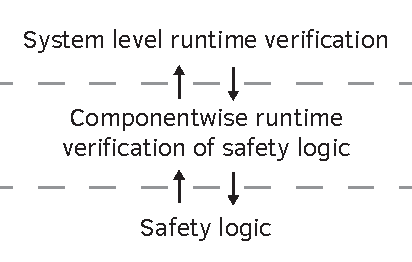
\includegraphics[width=0.75\linewidth]{include/figures/chapter_6/overview_1}
\end{minipage}

\section{Architecture}
	\subsection{Total view}
	\label{sec:case_study:total_view}
	Itt átvesszük a hardware alapjait, hogy egyáltalán miről van szó, hogy néz ki, mit tud.
	\subsection{Hardware}
	Itt az arduino alapú vezérlést emelném ki röviden, az ezzel felmerült problémákat, illetve a jövőbeli fejlesztések rövid bemutatását.

\section{Concept}
	A koncepció magyarázata, szép összefoglaló ábrával, és annak az összefoglalása, hogy mit tudunk ezzel elérni.

\section{Computer vision as a source of information}

\subsection{Hardware}
\label{sec:case_study:hardware}

In case of a computer vision (\textls{CV}) based approach, it is critical to choose the appropriate hardware. We had two parameters in the selection of the camera: height above the board, and \textls{FOV}.

\begin{dfn}
	Field of View (\textls{FOV}) is the extent of the observable world that is seen at any given moment. See \cref{fig:case_study:fov} for visual explanation.
\end{dfn}

\begin{figure}[h]
	\centering
	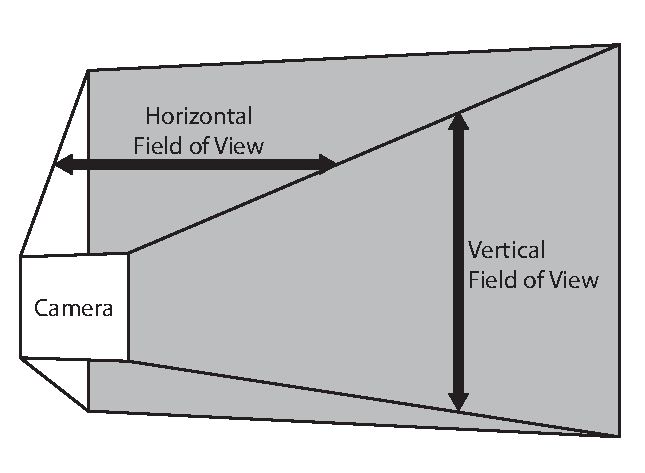
\includegraphics[width=0.5\linewidth]{include/figures/chapter_6/opencv_1}
	\caption{Visual explanation of \textls{FOV}}
	\label{fig:case_study:fov}
\end{figure}

These parameters are coupled, the higher the camera the less FOV we need. Most of the cameras on the market have horizontal FOV values approximately \ang{60}.

\begin{example}
	The board is 2.8~\si{\meter} wide. So if we assume we have a camera with a \ang{60} \textls{FOV}, using the result of \cref{equ:case_study:board_fov}, we need to place the camera 242 centimeters high. This would be is impossible to realize with average ceiling heights.
	\begin{equation}
		\label{equ:case_study:board_fov}
		242.48~\si{\centi\meter} = \frac{140~\si{\centi\meter}}{\tan(\ang{30})}
	\end{equation}
\end{example}

Our chosen \textls{FOV} became \ang{120}, because the cameras with these \textls{FOV} values are inexpensive, and easy to find. With a placement height of 120~\si{\centi\meter}, we can fully assemble the project virtually in any room.

\subsection{Computer vision}

One key point of this study from technological viewpoint is computer vision. It is a non intrusive add-on to the existing hardware, which allows us to monitor the board with fairly big precision and reliability, if the correct techniques and materials are used.

\subsection{Introducing to OpenCV}

We needed a fast, reliable, efficient library to use with the camera, and develop the detection algorithm. Our choose was the OpenCV\footnote{\url{http://opencv.org/}} library, which is an industry leading, open source computer vision library. It implements various algorithms with effective implementation in mind e.g., using the latest streaming vector instruction sets. The main programming language -- and what we used -- is \textls{C++}, but it has many binding to other popular languages like Java, and Python.

\subsection{Marker design}

One of the steps of the \textls{CV} implementation was the design of the markers, which should provide an easy detection, and identification of the marked objects.

The first step was to consider the usage of an external library, named \textls{ArUco}\footnote{\url{http://www.uco.es/investiga/grupos/ava/node/26}}. This library provides the generation (see \cref{fig:case_study:aruco_markers}), and detection library of markers.

\begin{figure}[h]
	\centering
	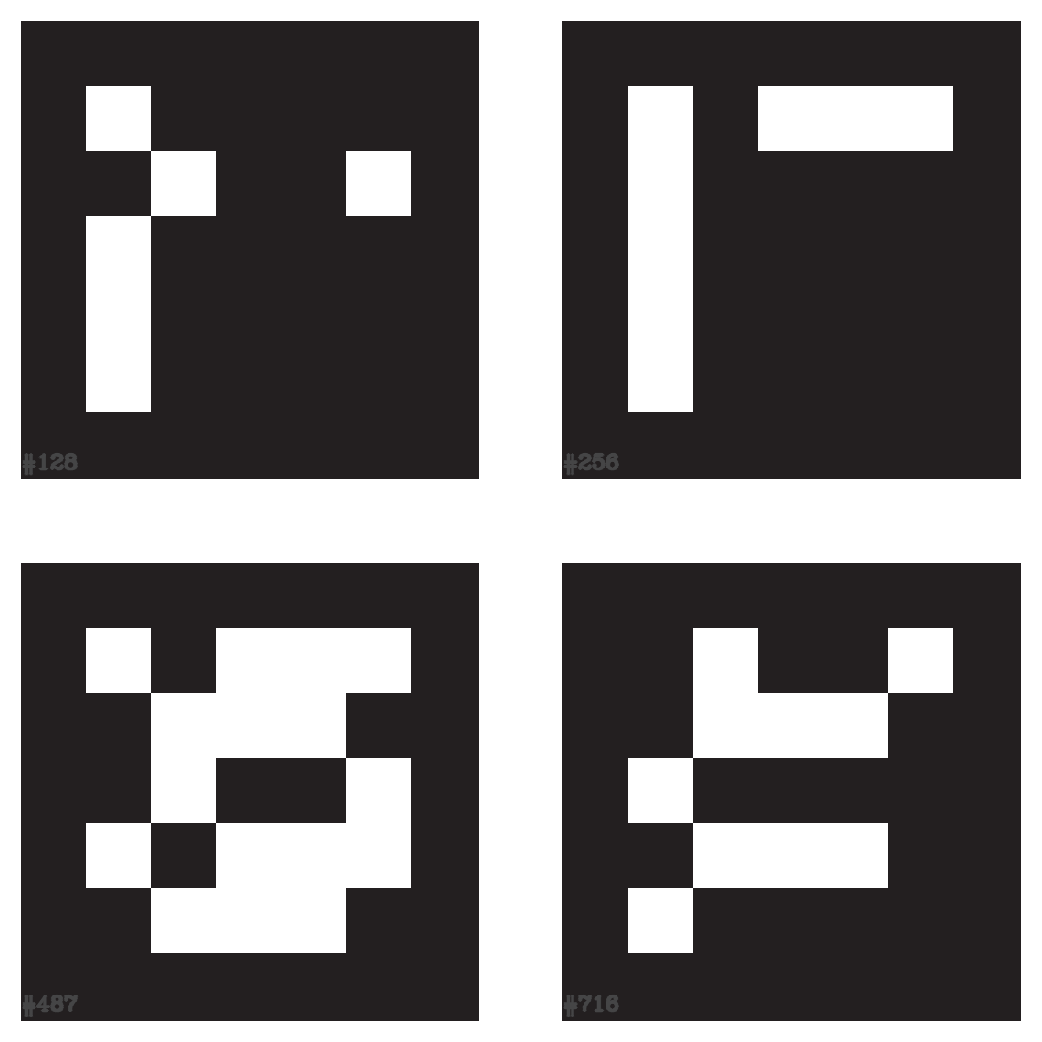
\includegraphics[width=0.35\linewidth]{include/figures/chapter_6/opencv_2}
	\caption{Example markers generated by \textls{ArUco}}
	\label{fig:case_study:aruco_markers}
\end{figure}

The problem with the library was the lack of tolerance in quality, and motion blur. Other limiting factor is the shape of the marker. A square marker scaled up to provide good visibility for the camera 120~\si{\centi\meter} above the board extends greatly over the width of a railway car. Because these negative properties of the existing libraries, we implemented a marker detection algorithm for our needs.

After the implementation was in our hands, we could make markers which suits our needs. The optimal marker covers the railroad car. This means the marker is narrow and long to fill the top dimensions of the car, but not exceed it.

As explained in \cref{fig:case_study:opencv_math}, circular patterns are well suited for these applications. The final design consists two detection circle, and a color circle for identification between the detection circles.

\begin{figure}[h]
	\centering
	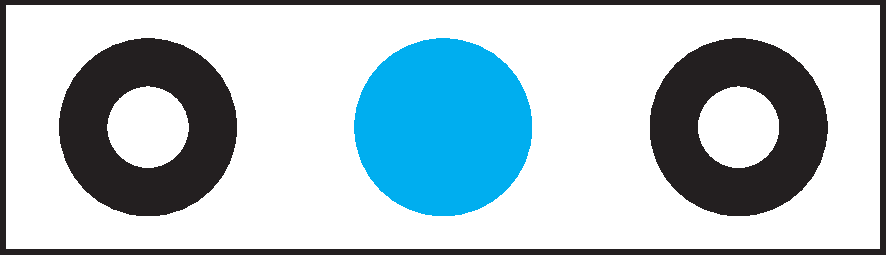
\includegraphics[width=0.75\linewidth]{include/figures/chapter_6/opencv_3}
	\caption{The final marker design}
	\label{fig:case_study:marker}
\end{figure}

\subsection{Software}

\subsubsection{Mathematical solution}
\label{fig:case_study:opencv_math}

Dimensions mentioned in \cref{sec:case_study:total_view} cause various environmental lighting conditions across the board. This is a challenging problem, because we must detect every circle despite we defined it as a perfect black circle, and every maker have its own lighting condition. 

This problem, and the fact that these markers have perspective distortion when they are near to the visible region of the camera motived us to develop a processing technique coming from controlling theory.

This method is the commonly used technique of transforming and processing a signal -- in our case a picture -- in frequency domain.

\subsubsubsection{Convolution method}



\subsubsection{\textls{CPU} implementation}
Az első implementáció gyors bemutatása.
\subsubsection{\textls{CUDA implementation}}
A GPU által gyorsított verzió bemutatása, mit tapasztaltunk ennek során, hogyan segített a fejlesztésben.

\section{Physical - logical mapping}
	\subsection{Elements of physical mapping}
		Az általunk használható architektúra részletes bemutatása.
	\subsection{Elements of logical mapping}
		Azoknak az elemeknek, elképzeléseknek az áttekintése, amik szerepelhetnek a modellünkben, még teljesen független módon.
	\subsection{Introducing to EMF}
		Az EMF bemutatása röviden.
	\subsection{Building the EMF model}
		Az elkészült EMF metamodell bemutatása, és összevetése az elképzelésekkel.
	\subsection{Introducing the IncQuery}
		Az IncQuery bemutatása.
	\subsection{Building the IncQuery patterns}
		A biztonsági lokikai patternek bemutatása.